\documentclass[a4paper,10pt]{article}
\usepackage[utf8]{inputenc}
\usepackage[margin=1.5cm]{geometry}
\usepackage{amsmath}
\usepackage{listings}
\usepackage{tikz}
\usepackage{siunitx}
\usepackage{pgfplots}
\usepackage{scrextend}
\usepackage{hyperref}
\usepgfplotslibrary{units} % Allows to enter the units nicely

\title{Codegeneratoren}

\author{
Sebastian Geiger\\ \small{Twitter: @lanoxx} \\ \small{Email: sbastig@gmx.net}
\and
Christian Hotz-Behofsits\\ \small{Twitter: @inkrement} \\ \small{Email: christian.hotz-behofsits@wu.ac.at}
\and
Dominik Pichler\\ \small{Twitter: @PicDom} \\ \small{Email: dpichler90@gmail.com}
}

\lstset{ %
  %backgroundcolor=\color{background},   % choose the background color; you must add \usepackage{color} or \usepackage{xcolor}
  basicstyle=\small\ttfamily,        % the size of the fonts that are used for the code
  %commentstyle=\color{mygreen},    % comment style
  %frame=lines,                    % adds a frame around the code
  columns=fixed,
  %keywordstyle=\color{blue},       % keyword style
  language=Java,                 % the language of the code
  numbers=left,                    % where to put the line-numbers; possible values are (none, left, right)
  numbersep=5pt,                   % how far the line-numbers are from the code
  %numberstyle=\scriptsize\color{mygray}, % the style that is used for the line-numbers
  showspaces=false,                % show spaces everywhere adding particular underscores; it overrides 'showstringspaces'
  showstringspaces=false,          % underline spaces within strings only
  showtabs=false,                  % show tabs within strings adding particular underscores
  %stringstyle=\color{mymauve},     % string literal style
  tabsize=2                       % sets default tabsize to 2 spaces
}


\sisetup{
  round-mode          = places,
  round-precision     = 2,
}

\begin{document}

\maketitle

\begin{abstract}
This is a short summary of the topics that are tought in \emph{Codegeneratoren}. Code generators are the backend part of a compiler
that deal with the conversion of the machine independent intermediate representation into machine dependent instructions and the various
optimizations on the resulting code. The first two sections deal with prerequisits that are required for the later parts. Section 1
discusses \emph{computer architectures} in order to give a better understanding of how processors work and why different optimizations
are possible. Section 2 discusses some of the higher level \emph{optimizations} that are done before the code generator does its work.
Section 3 discusses \emph{instruction selection}, which conserns the actual conversion of the intermediate representation into machine
dependent instructions. The later chapters all deal with different kinds of optimizations that are possible on the resulting code.

We have written this document for studing purposes only. Please make a commit@github, if you find errors or mistakes.
\end{abstract}

\newpage
\tableofcontents
\newpage

\section{Computer architectures}
Codegenerators are dependent on the computer architecture they are designed for. Therefore a comprehensive understanding of the different
concepts of computer architectures is requried. The Computer Architecture it self is defined as the attributes and behaviour of a computer seen by a machine langage programmer (e.g. instruction set \& format, adressing modes, operation codes and all registers and memory loctions that my be manipulated by a machine language programmer). In contrast, a specific \emph{implementation} defines the actual hardware structure and logic design and is intended to have a much shorter lifetime\cite{alpha}.

This capter can be roughly split into two main aspects: \textbf{microarchitectures} and \textbf{Instruction Set Architectures} sometimes abbreviated \emph{ISA}. The concept of \textit{microarchitectures} referes to the hardware part
of a processor, that is its different parts such as execution units, pipelines, caches and such. The instruction set architecture defines
the interface between the processor and its users (usually assembler programmers or compiler writers). It is easy to see that a
codegenerator is dependent on the instruction set architecture it was designed for. For example a different codegenerator is needed for
CISC and RISC computers. But a codegenerator developer also needs a good understanding of the underlying microarchitecture in order to
better optimize the generated code. An example for such optimizations is the use of instruction level parallelism or code scheduling to
achieve a higher pipeline utilization. Below the most important concepts of microarchitectures and ISA are explained.

\subsection{Microarchitectures}
Each processor is composed of many different hardware parts, that are all responsible for different things. The following list gives an
overview of the most important parts and their functions:
\begin{description}

 \item[Register/ Register file] A processor register is a small but fast storage as part of a digital processor. Depending on the architecture these registers are fore general purposes or just for special values (e.g. integer, floating point). A register file is a array\footnote{"Compilers can deliver substantial perfomance gains when given 32 registers instead of 16[per register file], but there is no clear evidence of similar gains when going to 64 registers."\cite{alpha}} of registers and can be combined or split/partitioned (different files for different purposes). Especially if \emph{multiple issue} support is intended (e.g. VLIW) the register files are likely split. Although a combined approach is more flexible and easier for the compiler to handle.
 \item[Caches] Store some of the program code and data from memory to allow faster access. Separate instruction and data caches
       can allow simultaneous instruction and data access every cycle. Integrated Caches are especially important if only a small number of registers are available, to speed up memory usage. \emph{Nonblocking Caches} (a.k.a. \emph{Hit-Under-Miss-Cache}) are able to handle subsequent data requests, while waiting for results of former requests (used e.g. in Intel P6).
 \item[In/out of order execution] Realized by reorder buffers. Instructions are dispatched to the reorder buffer in-order but
       the execution units can execute the instruction out-of-order. PowerPC 604 uses out-of order execution \cite{powerpc}.
 \item[Register renaming] Register renaming minimizes architectural resource dependencies, namely WAW
       \footnote{\label{footnote-waw}WAW and WAR are abbreviations for data dependencies and are explained in Section \ref{sec:graphs}.}
       and WAR\footref{footnote-waw} dependencies. If instructions are executed out-of-order, then it maybe the case
       that a result needs to be written into a register while an earlier instruction still needs the old value. By renaming the register
       and temporarily storing the new result in a different register the data dependency between those instructions can be broken up. On
       the microarchitectural level \textbf{rename buffers} are used to implement register renaming. Register renaming can also be used to optimize the execution of some instructions (e.g. the FXCH command in Intel's P6 needs no single cycle because it uses register renaming).
 \item[Precise interrupts] An interrupt (e.g. arithmetic exception, page fault) is precise if it leaves the system in a well-defined state:
 \begin{itemize}
   \item All instructions before the one that caused the interrupt are fully executed.
   \item All effects (e.g. register and memory modifications) from instructions after the one that caused the interrupt are undone.
 \end{itemize}
 Processors that do not have precise interrupts (e.g. Alpha AXP has only imprecise arithmetic exceptions but precise memory exceptions) are faster, easier to design but quite difficult to program. A reorder buffer (managed as FIFO queue), which kepps track of the instructions order
       and the state, can be used to implement precise interrupts\cite{powerpc}.
 \item[Reorder buffer] A reorder buffer is used to save and restore the original order and the states of instructions as they are dispatched
       to execution units. Reorder buffers are used to implement prceise interrupts, because they allow the processor to enforce in-order
       completion of instructions even though they maybe executed out-of-order by the execution units.
 \item[Completion stage] Important for precise interrupts. Also separates completion stage and write-back stage to support load-
       with-update instructions.
 \item[Branch prediction] A technique to avoid pipeline stalling. The processor predicts if a branch is taken and what its
       target address is before this information becomes available. If the prediction is correct then the pipeline continues to process
       with full through put. If the prediction is wrong, then the pipeline must discard all pending operations and restart at the branch or at the
       correct location.
 \item[Branch target address cache] Used to predict the target address of a branch or jump instruction. The BTAC is accessed
       with the fetch address and returns the target address.
 \item[Branch history table] Stores information about whether a branch was taken or not, depending on the complexity of the
       branch history table it is also possible to store patterns, such as, that a branch was only taken every second time.
 \item[Reservation station] Used to keep an instruction until its operands become available (The PowerPC 604 has two
       reservation stations for each execution unit). This way instructions can be dispatched even if their operands are not yet
       available.
 \item[Split Transaction Protocol] Allows a more efficient bus usage. While other techniques occupy the bus access while waiting for data, in STP it's not nessecary. First the address is provided, then the bus is released and only re-occipied if the results are present (used by Intel P6). This simplifies the setting of an Multiprocessor (MP-) System, where the same bus is used by multiple processors.
 \item[Serialization] Is used to delay the execution of certain (expensive) instructions (e.g move to and from special purpose registers). So it's possible to prevent the speculative execution of expensive instructions and minimized the penalty of serialized instructions.
 \item[Superscalar architecture] A superscalare processor executes more then one instruction during a clock cycle by
       simultaneously dispatching multiple instructions to redundand functional units on the processor, this can include different
       functional units such as branch, integer, multiply, floating-point units, but also redundand units
       of the same type such as four integer units. Examples for superscalar architectures in common processors are:
	\begin{itemize}
	    \item Hyperthreading (duplicates register space for the thread context)
	    \item Multiple execution units (often combined with out of order execution)
	\end{itemize}
  \item[Pipelining] Increases the \textbf{frequency} of the processor, but also the \textbf{latency}, one instruction requires
multiple clock cycles. Instructions handling is split into several stages (e.g. Intel P6 has 12 steps) where each stage can handle one instruction at a time. The
instruction passes through several stages before its computation is complete. Typical stages are: (Fetch, Decode, Dispatch, Execute,
Write-back, etc.)\cite{powerpc}. The latency usually covers only the execution stage. Example: In the first cycle an instruction is fetched by the
fetch stage, then in the next cycle an new instruction is fetched by the fetch station and the first instruction moves on to the decode
station where it is decoded.

	\begin{itemize}

    \item \textbf{Pipeline hazards:} are the drawbacks of pipelining and are caused by the increased latency of
instruction results. Such a hazard often appears if a second instruction depends on the result of a first instruction. It can be solved
with different techniques such as out-of-order execution. Another problem appears in combination with branch prediction. If a branch is
wrongly predicted, then the pipeline becomes invalid and must be restarted, which leads to a penalty of several cycles.

    \item \textbf{Deep Pipelining:} If the pipeline uses more steps (aka. is "deeper"), each step gets less complicated and allows a higher frequency. But this has also some drawbacks. On a failure (e.g. division by zero or miss prediction) more steps have to be discarded, which costs time (Intel's P6 tries to counteract by using sophisticated branch prediction). Furthermore deep pipelining requires some expensive component-properties (e.g.  very large on-chip caches, wide data bus, fast memory systems)\cite{powerpc}.

    \item \textbf{Pipeline bypass:} A way to prevent pipeline hazards is a pipeline bypass. This allows a value that was computed by the
previous instruction to be read by the next instruction without the need to wait until the instruction has gone through the complete and
writeback stages.

	\end{itemize}

\end{description}


The processor performance depends on\cite{powerpc}:
\begin{itemize}
\item Number of instructions in a task
\item Number of cycles a processor takes for to complete the task
\item processor's frequency
\end{itemize}


\subsection{Instruction Set Architectures}
An instruction set architecture defines the programming interface of the processor. It includes aspects such as instructions, registers,
data types and memory access, as well as interrupt handling and exception handling. The instruction set architecture also defines how
external I/O is done. Common instruction set architectures are:
\begin{description}
 \item[RISC] \textit{Reduced Instruction Set Computer)} Referes to a load-store architecture with fixed width instructions.
 \item[CISC] \textit{(Complex Instruction Set Computers)} Architecture which allows complex memory access, supports complex instructions
       and variable width instructions.
 \item[VLIW] \textit{(Very Long Instruction Word)}/ \textbf{EPIC} \emph{(explicitly-parallel instruction)}. Both Architectures combine multiple instructions for parallel execution and are quite similar. In contrast to superscalar architectures it has to be explicitly defined which instructions should be executed in parallel. This is done by the compiler which generates "bundles" of instructions, whereas the nop operation is often used to satisfy instruction placement constraints (this leads often to increased code size in case of VLIW).
\end{description}

There are two very important differences between CISC and RISC, one is the way memory access works, the second is the instruction width.
RISC uses a load-store architecture in which instructions that operate on the memory are only used to load data into registers or store
data in memory, while all computation happens on values in registers. CISC on the otherhand also allows operations to modify data directly inside
the memory. The second big difference is the width of instructions. RISC has a fixed instruction width (such as 4 bytes) where as CISC
has a variable instruction width. It is also important to note that pipelining and superscalar architectures can be problematic on CISC processors due to the complexity of CISC instructions.


\subsubsection*{Endianness and Data units}
The endianness refers to the order of the bytes. Some architectures (e.g. Alpha AXP) use little-endian view (byte 0 is the low byte of an integer) others big-endian (most significant bit is stored in the lower memory address).

\begin{description}
\item[Byte] 8-bit datum.
\item[Word] is a fixed-sized piece of data handled as a unit by the instruction set or the hardware of the processor. The size depends on the specific architecture.
\end{description}

\subsubsection*{Binary Translation}
Binary Translation is the emulation of a specific instruction set by another one based on binary code. There are two types (dynamic and static) whereby only dynamic binary translation is important in this context. Dynamic techniques can furthermore divided in those based on software and hardware:

\begin{itemize}
\item \textbf{Hardware:} (As already mentionend) x86 Intel CPUs (since P6) translate complex CISC x86 instructions to more RISC-like internal Microcode instructions.
\item \textbf{Software:} DEC provided translation tools to help users migrate from the VAX to the Alpha RISC architecture.
\end{itemize}

\subsubsection*{Instruction level parallelism}
Instruction level parallelism (ILP) referes to the fact that under the right conditions (independent instructions and/or right hardware) instructions can be
executed simulaneously (Multiple Instruction Issue). It is used as a measure for the degree of parallelism in a given program. There are different techniques to
exploit this inherent parallelism in programs.
\begin{itemize}
 \item \textbf{Static Multiple Issue} Here the paralellism is forced by the compiler and therefore it is explicit. This allows easier hardware and execution is faster (no time required to identify parallelism at execution time). Cause of the placement constraints the binaries are often a bit larger in size. Examples: \emph{SIMD} \& \emph{VLIW}

 \item \textbf{Dynamic Multiple Issue:} the ILP can be exploited by many techniques of the microarchitecture such as \emph{instruction pipelining},
 \emph{superscalar execution} (feature of all current x86 architectures), \emph{out-of-order exectuion}, \emph{register renaming} and \emph{branch prediction}.
\end{itemize}

\subsection{Concepts and Instructions}
In Computer architectures exists a lot of different concepts. Some are tied to a specific Instraction Set Architecure (e.g. Microcodes) and others like SIMD are not. In the following subsections you will find descriptions of some more or less important concepts.

\subsubsection{CISC}
\begin{description}
\item[micro-operations] To reduce the complexity of CISC-operations, micro-operations are introduced, where instructions are first converted
into one or more micro-operation and are then dispatched and executed by the processor (Intel's $\mu Ops$ or AMD's \emph{ROPs}). These micro-operations have often a lead/store archtiecture similar to RISC. This fact however does not turn a CISC processor
into a RISC processor, it is just an implementation detail of the microarchitecture of CISC processors.
\end{description}


\subsubsection{RISC}
  \begin{description}
  \item[PRISM] This is a hardware abstraction layer used by some RISC architecutres (e.g. Alpha AXP) to support different operating systems (OS). Each OS has it's own \emph{PALCode (Alpha Machine Code)} running in a special mode (controlled entry points, interrupts turned off and access to real hardware registers) \cite{alpha}. It covers features like interupt delivery and return, exceptions, error handling, memory mamangement and context switching. Access to physical hardware resources (e.g. memory) is mediated by PALcode routines.
  \item[Branch Delay Slot] is the name of the command next to a conditional branch command. It's used to provide better utilization of the pipeline: it will be executed anyhow and helps to pass the waiting period till the result of the branch is known. It does not work well with multiple instruction issue, because a lot of delay slots would be needed to be efficient\cite{alpha}.
  \item[Suppressed (or Skipped) Instructions] allow that the executions of one instruction conditionally surpresses the following one. It's difficult to handle this in a multiple issue setting, because a non-replicated state is represented by one or more suppresion bit(s)\cite{alpha}.
  \item[(single) Byte load/store Instructions] Reading or Writing multiple bytes or to rw a single byte in memory can be a performance bottleneck. These operations require a extra byte-shifter in the speed-critical load and store paths. Byte stores and loads can be substututed by a load/shift or a load/modify/store sequences.
  \end{description}

\subsubsection{ISA-independent}
\begin{description}
\item[SIMD Instructions] (Single instruction, multiple data)
\begin{quote}
    \textit{''SIMD instructions provide a form of vectorization where a large machine word is viewed as a vector of subwords and the same
    operation is performed on all subwords in parallel``} \cite{simd}.
\end{quote}
For example a SIMD instruction could operate on vectors with a size of 128bit and the data elements could be 16bit wide (short integers).
An vector of a SIMD instruction would therefore contain eight data elements. If the processor supports a SIMD \lstinline{add} instruction
this allows two vectors of 8 elements to be added into a vector with 8 elements with a single instruction. When the SIMD instruction is
executed, the processor effectively performs eight add operations simulatenously. In that regard SIMD instructions are similar to
superscalar processors, but have a much higher degree of parallelism.

The SIMD concept is not tied to a particular ISA but can be added to RISC, CISC or even VLIW architectures. On the microarchitectural
level the processor has special SIMD registers and SIMD execution units to support the different SIMD instructions.
\end{description}


\subsection{Examples}
The \textbf{Alpha AXP} is microprocessor with a RISC instruction set. It supports precise memory interrupts but only imprecise arithmetic exceptions. It was built targeting a lifespan of 25 years while providing easy adaption of the VAX/VMS user base (e.g. binary translation). It uses PALCode to enable support for a wide range of operating systems without the burden of biasing toward a specific computing style. The architecture avoids usage of some components that would conflict with the multiple instruction issue (e.g. branch delay slots and common register slots).

The \textbf{Intel P6} is a CISC architecture to preserve combatibility to former products. It uses microcodes with a load/store-architecture to handle complexity and has a pipelined processor providing precise interrupts (a reorder buffer is used to ensure the right instruction order). The pipeline has 12 steps and is therefore quite "deep". To prevent hazards a sophisticated branch prediction is build in. Furthermore Split Transaction Protocol in combination with Nonblocking Caches are used to allow performant Multi Processor Support.

%% TODO: coherency of cache (end p.7ff)?
%% TODO: bus interface and memory queues (p8)
The \textbf{PowerPC 604} is a superscalar RISC processor joinly developed by Apple, IBM and Motorola. A target was a low cost chip with support of (for this time) quite high clock rates, therefore a deep pipleline (6 stages: fetch, dispatch, execute, completion and writeback) is utilized. Furthermore precise interrupts, register renaming, branch prediction, serialization and a speculative execution is supported. The 604 provides separate nonblocking instruction and data caches.

\section{Optimizations}
\label{sec:optimization}
This section describes high-level optimizations that are performed by the compiler on the intermediate representation of a program. At
this point the code is still machine independent and instruction selection has not yet been performed.

\subsection{Static Single Assignment}
Static single assignment (SSA) is an optimization required to enable most other optimizations, it is a form where each variable has only
a single value assignment. Additionally every variable must be defined before it is used. Every code can be transformed into SSA form by
adding indexes to variables. For example

\parbox{10cm}{
\begin{flalign*}
    i &= 5 + 7 &\\
    z &= 8\\
    i &= i + z
\end{flalign*}
}

\noindent becomes:

\parbox{10cm}{
\begin{flalign*}
    i_1 &= 5 + 7 &\\
    z &= 8\\
    i_2 &= i_1 + z
\end{flalign*}
}

\noindent When dealing with branches, $\varphi$-nodes are added to merge variables from separate branches:

\begin{lstlisting}[xleftmargin=.5cm,numbers=none,mathescape=true,columns=flexible,basicstyle=\ttfamily]
if(a)
    $i_1$ = 10
else
    $i_2$ = 20
$i_3$ = $\varphi(i_1,i_2)$
\end{lstlisting}

\subsection{Graph structures and memory dependencies}
\label{sec:graphs}
Graph data structures are also required for most optimizations and contain information about data dependencies between instructions, they are also often called \textbf{dependency graphs}. In general graphs can be separated into two categories: acyclic graphs and cyclic graphs. \textbf{Acyclic graphs} are often used to model code inside basic blocks\footnote{ The concept of basic blocks is introduced in the compiler construction lecture and refers to a block of code with only one entry and one exit point. That means in particular that basic blocks cannot contain loops or branches.
} or extended basic blocks. On the otherhand \textbf{cyclic graphs} are usually used to model loops or recursion and usually extend over a whole proceedure and not just a basic block. In such graphs instructions (or operations) are represented as vertices and data dependencies as edges. Depending on where the graph is used vertices and edges can be annotated with additional information such as delayes between instructions. Data-dependence testing is required for any form of automatic parallelism detection (i.e. determine, when two operations of a loop can be executed in parallel).\\

The data dependencies that form the edges of a graph can be categorized into three kinds of dependencies:

 \begin{itemize}
     \item true dependency, flow dependence or \textbf{read after write} (RAW). $S_{1}$ must be executed before $S_{2}$. $S_{3}$ and $S_{2}$ can be executed in parallel.

\parbox{5cm}{
  \begin{flalign*}
    S_{1}: A &= B + C & \text{write A}\\
    S_{2}: D &= A + 2 & \text{read A}\\
    S_{3}: E &= A * 3 & \text{read A}\\
  \end{flalign*}
}

	\item anti-dependency or \textbf{write after read} (WAR). $S_{1}$ uses the "old" value of B, therefore must be executed before $S_{2}$. Relation goes from the use to the assignment.

\parbox{5cm}{
	\begin{flalign*}
	  S_{1}: A &= B + C & \text{read B}\\
	  S_{2}: B &= D / 2 & \text{write B}
	\end{flalign*}
}

     \item Output dependency or \textbf{write after write} (WAW). $S_{1}$ MUST preced $S_{3}$, if not, A would have a wrong value afterwards.

\parbox{5cm}{
	\begin{flalign*}
	 S_{1}: A &= B + C &   \text{write A}\\
	 S_{2}: D &= A + 2 \\
	 S_{3}: A &= E + F &    \text{write A}
	\end{flalign*}
}

 \end{itemize}

Flow of control must also be taken into account, because of the different branches of e.g. an if-statement. $S_{2}$ and $S_{3}$ would have RAW dependence, but because of the if, this can never happen. Because the actual flow is not known at runtime, "unnecessary" relations will also be taken into account, all dependencies between $S_{1}$ and $S_{4}$, $S_{2}$ and $S_{4}$, $S_{3}$ and $S_{4}$ will be calculated.

\parbox{5cm}{
	\begin{flalign*}
	 S_{1}: A &= B + C\\
     & C_{1}: if (X >= 0) \ then\\
	 S_{2}: A &= 0 \\
     else \\
	 S_{3}: D &= A \\
     endif \\
     S_{4}: A &= D*2
	\end{flalign*}
}

Therefore many compilers add a dependence from the if-statement (\textbf{control dependence-relation}) to the data-dependence graph, e.g. $C_{1}$ - $S_{2}$, to find which statements can be reordered or find cycles in the graph.\\

\textbf{Data-dependence inside loops} means relations between statements and between instances (instance of statement during on iteration step) of statements. The dependence can stay in the same iteration, flow from iteration i-1 to iteration i, or flow from iteration i+1 to iteration i.\\

 \begin{itemize}
 	\item stay in the same iteration\\

\parbox{5cm}{
	  DO I = 2,N\\
	  A(I) = B(I) + C(I)\\
      D(I) = A(I)\\
      end do
}

	\item flow from iteration i-1 to i\\

\parbox{5cm}{
	  DO I = 2,N\\
	  A(I) = B(I) + C(I)\\
      D(I) = A(I-1)\\
      end do
}

     \item flow from iteration i to i+1\\

\parbox{5cm}{
	  DO I = 2,N\\
	  A(I) = B(I) + C(I)\\
      D(I) = A(I+1)\\
      end do
}

 \end{itemize}

If there are no cycles in the dependency graph, the loop can be completely vectorized. To use multiple processors, the iterations are partitioned a assigned to the processors (spreading). Important is to avoid synchronization and that the processing leads to an equal result compared to serial processing.\\
If unnecessary relations are added to the data-dependency graph, the potential for parallelism discovery is heavily decreased.
Many of the optimizations that are introduced in this and the later chapters require a detailed knowledge of the data dependencies between instructions.\\

\subsection{Machine independent optimizations}
Machine independent optimizations are performed on the intermediate representation and are independent of the machine (i.e the instruction
set architecture) being used.
\begin{itemize}
 \item Scalar optimizations:
 \begin{itemize}
     \item \textbf{Constant Evaluation:} resolves expressions of multiple constans such as 5+7 which is resolved to 12
     \item \textbf{Constant Propagation:} propagates the constant to places in the code where variables refer to constants
     \item \textbf{Copy Propagation:} replaces the use of a variable with the use of another variable of equal value
     \item \textbf{Common subexpression elemination:} Opposite of \textbf{rematerialization}
     \item \textbf{Scalar expansion:} Propmote scalar to vector/array inside loop (used in SIMD and VLIW)
     \item \textbf{Strength reduction:} replaces expensive instructions by cheaper ones (eg. replace $5*a$ with $a>>2+a$ since shift and add are cheaper than multiplication). Another meaning of strength reductions can concern address optimizations in connection with indiction variables.
 \end{itemize}
 \item Progam optimizations:
 \begin{itemize}
     \item Dead code elemination (reachable vs. useless code elimination)
     \item Function inlining (Speed) vs. Procedural abstraction (Code size)
     \item Tailcall elimination: Resolves recursion into iterative loops (very common in logic programming)
     \item Peephole optimization (very small optimizations 2-3 instruction, hard to analyze)
 \end{itemize}
 \item \textbf{Induction variable} elimination: is an optimization that tries to identify and remove the induction variables inside loops and optimize array address calculation.
  \begin{itemize}
  	\item Ind. Var: Variables in loops whose successive values form an arithmetic progression (e.g. index of a loop, function of the loop index variable, self-dec/increment)
    \item used in array subscript expression, e.g. A(i+1)
    \item The improved loop uses pointer arithmetic instead of an index variable
    \item Invariant code motion moves code that does not depend on the loop body out of the loop body
    \item Use information about induction variable for optimization
    \item some variables look like ind. vars. but does not qualify, e.g. if a variable is used before it is assigned and the values assigned are not used until the next iteration. (\textbf{wrap-around variable}).
  \end{itemize}
  \item \textbf{Loop optimizations}:
     \begin{itemize}
     \item Loop interchange (change inner and outer loop without affecting the outcome), the inverse function is still loop interchange. Not always possible and has to be determined with data dependence graphs. Often used for loop vectorization. It is also possible to put a concurrent lop on the outside to use multiple processors.
     \item Loop fission vs. Loop fusion
     \begin{itemize}
     	\item fission: break a single loop into several adjacent loops. Two statements will stay in the same loop, if there is at least one variable or array referenced by both. Fission by name ("distribution of name partitions") is used to enhance memory hierarchy performance
        \item fusion: transform two adjacent loops into a single loop. With data-dependence test more loops can be fusioned than with standard techniques. Data-dependency relations must not be violated. Used to reduce overhead of loops. Combine separate loops, if they refer to the same set of variables, with the same goal as fission by name - compiler would have a larger loop with the benefits of loop fusion, but still have improved memory hierarchy performance that comes from only refering to a small set of arrays in the loop.
        \item Compiler must not fusion loops which have been fissioned.
     	\item Loop peeling is special case of loop splitting that peels of one or more iterations from the beginning or the end of the loop and performs these operations separately before or after the loop.
     \end{itemize}
     \item Loop collapsing (transforms two nested loops into a single one) vs. Strip mining. Used to increase the effective vector length for vector machines. (Bsp. [4] S. 41) General version is useful for parallel computers.
     \item Strip mining transforms a single loop into a doubly nested loop where the outer loop is incremented by a certain block size
     and the inner loop is incremented by one:
     \begin{lstlisting}
	for(int j=0; j<N; j+=32) {
	    for(int i=j; i<min(j+31, N); i++) {
	        //loop body
	    }
	}
     \end{lstlisting}
     The block size depends on characteristics of the target machine., e.g. vector register length or cache memory size. For vector machines, the inner loop will be vectorized. For parallel machines the outer can be concurrentized.
     \item Loop vectorization (SIMD, VLIW): The compiler analyzes the dependence graph and if no loops are found it can make use of
           special vector instructions of the target processor.
     \item Loop concurrentization: Loops are split into several partitions and each partition is computed on a different processor
           concurrently.
 \end{itemize}
 \item Reorder transformation (like code scheduling but higher level, e.g. compiler frontend not backend). Uses sophisticated dependency
       analysis.
\end{itemize}

\section{Instruction selection}
Instruction selection is a process which transforms the the compiler's intermediate representation of the program into object code (target-dependent machine instructions), by selecting a machine instruction for each computation. The resulting object code after instruction selection is therefore machine dependent and optimized for various compiler objectives. Instructions may have associated costs and the goal of instruction selection is to find a sequence of instructions, which have minimal costs.

There exist several implementations for instruction selection, which are presented in the following sections.
\subsection{iBurg}

iBurg is a variant of Burg - a code-generator generator\\

\textbf{Burg} (was not discussed in the lecture) uses BURS(bottom-up rewrite system) theory, to move the dynamic programming to compile-compile time. BURS table generation is more complicated, but generate optimal code in constant time per node.\\

\textbf{iBurg} is an improved version of Burg. It reads a Burg specification and writes a matcher (hard-coded) that does dynamic programming at compile time. Its main advantage is that it is simpler to implement (about 700 lines of code) and that it admits larger class of tree grammars. Although iBurgs matchers a slower than BURS' matchers, they are more flexible and still practical.\\

Burg computes costs that must be constant, because dynamic programming is done at compile-compile time and iBurg at instruction selection time (compile time/code-auswahl zeit/laufzeit). Therefore in theory iBurg could support dynamic costs (e.g. concrete values of immediates), but does not do so in practice for backwards compatibility with Burg. Instructions are selected through tree pattern matching and dynamic programming. The goal of tree pattern matching is to find a minimal cost cover for the data flow tree that represents the operations of the intermediate language.\\

\begin{itemize}
	\item In a tree, there are terminals and non-terminals and rules. Non-Terminals are on the left side of rules. 		\item Terminals are the operators of subject trees with a fixed arity, e.g. ADDI for integer addition, and on the right side of rules. An arity of zero means, that it is a leave.
	\item Each non-terminal denotes a tree.
	\item rules define tree patterns. Each rule has a unique positive external rule number (are used to report the matching rule to a semantic action routine) and have an optional integer "cost" (0 by default)
	\item a chain rule is a rule whose pattern is another non-terminal
\end{itemize}

Both Burg and iBurg generate functions to \textit{label} (first pass) and \textit{reduce} (second pass) subject trees. \textit{label} makes a bottom-up left-to-right traversal to compute rules that cover the tree with minimum costs, if there is such a cover. Each node is labeled with (M,C) where M is a matching rule and C are the costs and the costs are summed up. Nodes are only annotated with (M,C), if C is less than all previous matches for the non-terminal on the left-hand side of the rule M. Once labeled, a subject tree is \textit{reduced} by traversing it from top down and performing appropriate semantic actions (e.g. generating and emitting code).\\

Burg does all dynamic programming at compile-compile time and annotates each node with a single, integral state number which encodes all of the information concerning matches and costs. iBurg does the dynamic programming at instruction-selection-time/compile time/code-auswahl zeit/laufzeit and annotates nodes with data equivalent to (M,C). Its state numbers are really pointers to records that hold these data.\\

Both Burg and iBurg use the non-recursive function \textit{state} to identify matches. iBurgs state function is straightforward (simple \textit{switch}-statements with if-statements for non-leaf cases until match is found) for tree pattern matching and generates hard-code. It's state numbers are pointers to state records, which hold vectors of the (M,C) values for successful matches. This saved computed states helps to retain flexibility of dynamic cost computations at nearly the of precomputed states like Burg has. If a match succeeds the resulting cost is computed and \textit{record} is called. A match is only recorded, if its cost is less than previous matches.\\

Further advantages of iBurg:
\begin{itemize}
	\item Definitions can be mapped into a compact range of integers and stored in minimum space in state records as bit fields.
	\item use little space for large specifications
    \item save time
    \item initialization costs are reduced.
    \item save time for leaves
    \item more compact approach to handling of chain rules
    \item generated state and label functions are easy to read and to debug
\end{itemize}

The reason why state is an integer which is casted to a pointer is, because there are problems with 64-bit architectures.

\subsection{BEG}
BEG stands for Back End Generator. It is not only used for instruction selection but also includes register allocation. The important
aspects of BEG are:
\begin{itemize}
	\item hard-coded
    \item use dynamic programming at compile time to identify a minimum cost-cover
    \item It is more advanced then iBurg
    \item Has a more powerful rule engine and supports \textbf{dynamic costs} and \textbf{conditions} for instruction selection.
    \item Can do \textbf{register allocation}, but only locally on basic block level
    \item Has two types of register allocation (on the fly, general register allocation)
\end{itemize}

\subsection{Dag-driven instruction selection with PBQP}
Another solution for instruction selection is the dag-driven instruction selection using SSA-Graphs (Single-Static-Assignment, as an intermediate representation of programs) and PBQP (for finding optimal instruction selection). Instruction selection is modeled as a partitioned boolean quadratic problem (PBQP) which is an NP-Complete problem.\\

\textbf{SSA form}: Each variable has a single assignment in the source code. If a variable $i$ has two assignments, it is splitted int $i_{1}$ and $i_{2}$.\\

\textbf{SSA graphs} are abstract representation of procedures in SSA form. Nodes in the SSA-graph are simple operations (e.g. load, store, arithmetic instr.,...) and incoming edges are the ordered arguments of an operation, outgoing one's are the result $\rightarrow$ so the data flow is modeled, but not the data flow through memory. That is, SSA graphs do not directly reflect memory dependencies (look below for an example). This can lead to cycles which must be broken up by adding potential data dependencies.\\

\textbf{PBQP}, a specialized quadratic assignment problem, is the instruction selection algorithm and tries to find a cost minimal assignment $h$ of variables $X$ to their respective domains $D$:
\[ h: X \rightarrow D\]
At the core of PBQP two functions are used, a local cost function (quality of the assignment) $c$ and a related cost function (quality of assignment for two related variables) $C$, the sum $f$ of both forms the cost of an assignment for variables to their respective domains:
\[ f = \sum c_i + \sum{C_{ij}} \]

The instruction selection with PBQP works like this. For each node $u$ in the input SSA-Graph there exists a variable $x_u$ which is mapped to an operation out of a list of possible operations for this node. (The domain of $x_{u}$ is the subset of base rules whose operations match the operation of the SSA node $u$) The possible operations are defined by a normalized graph grammar which consists of base rules(production from non-terminal to terminal) and chain rules (production from non-terminal to non-terminal). The local cost function is defined as a cost vector $c_u$ of $x_{u}$ that encodes the costs of selecting a base rule.\\
An edge in the SSA graph represents data transfer between the result of an operation $u$ (source of edge) and the operand $v$ (tail of the egde). To \textit{``ensure consistency among base rules and to account for the costs of chain rules''} the related cost function is modeled as a matrix $C_{uv}$ (Uebergangsmatrix von $u$ zu $v$). An element in the matrix corresponds to the costs of selecting a specific base rule from $x_{u}$ and from $x_{v}$. The values of $c_u$ and $C_{uv}$ are either \textbf{zero} for matching base rules, \textbf{infinite} for incompatible base rules or a value which is the \textbf{sum of transitive chain rule costs} in order to make two non-matching base rules compatible. In summary: \textit{``A solution of PBQP determines which base rules and chain rules are to be selected''} \cite{pbqp-instruction-selection}. There is also a parameter $w_{u}$ that is used as a parameter to optimize objectives like speed or space.\\

The PBQP based instruction selection also allows instruction selection for complex patterns that can have multiple results and cannot be expressed in terms of tree shape productions, e.g. ``div-mod'' (divide and modulo) or ``auto-increment'', however this can lead to cycles in the graph. Complex patterns can have multiple in-coming and out-going edges and cover multiple nodes in the SSA-graph at the same time.\\

\textbf{Complex patterns} for instructions with multiple outputs such as ``div-mod'' or ``auto-increment for pointers'' can cause cycles in the graph. This can happen if \textit{``a set of operations in the SSA graph is matched by a pattern for which there exists a path in the SSA graph that exits and re-enters the complex pattern within the basic block''} \cite{pbqp-instruction-selection}. This would imply that operations are executed on the target, before the values of the operands are available. The matcher must prohibit this cycle by finding a topological order among those patterns. Complex patterns are matched by enumerating the set of all viable instances of a complex pattern. In the resulting set two instances $p$ and $q$ within a basic block $b$ may have a dependency $p \prec_b q$, which can lead to the cycles mentioned above. Such cycles are broken up by adding additional constraints in the form of \textbf{cost matrices}, which \textit{'' constrain the solution space such that no cyclic data dependencies can be constructed in any valid solution``} \cite{pbqp-instruction-selection}.\\

As mentioned above, SSA-graphs do not reflect memory dependencies. However, the do have memory operations that impose data dependencies amon memory operations including $loads$ and $stores$. For example: a read-modify-write pattern such as $"add r/m32, imm32"$. \\
\begin{lstlisting}
  x = *p;
  *q = 1;
  y = x+2;
  *p = y;
\end{lstlisting}

If we assume that $p$ and $q$ might address the same memory locations, the anti-dependence between (1) and (2) and the output dependency between (2) and (4) must be ensured. To ensure a topological order among the chosen productions, the SSA-graph is augmented with additional edges representing potential data dependencies.\\

The extension of the instruction selector is mainly concerned about prohibiting cycles in the selection of patterns considering memory dependencies for the instruction selection\\

For \textbf{solving PGQP instances} two solvers are used:
\begin{itemize}
	\item A \textit{heuristic solver}, which solves a subclass of PBQP optimally in $O(nm^{3}]$, where $n$ is the number of discrete variables and $m$ is the maximal number of elements in their domains. It eliminates discrete variables until the problem is trivially solvable. The elimination requires reductions and if no reductions are applicable, the problem becomes irreducible and a heuristic $RN$ is applied which searches for local minima.
    \item An \textit{exponential branch-and-bound solver} searches the space spawned by the $RN-nodes$ of the problem. The space is pruned by a lower bound to speed things up.
    \item the results of the heuristic solver are nearly as good as the ones from the exact one.
\end{itemize}

An important difference between the different instruction selectors is when costs are computed. Burg do it at compile-compile time, where as and iBurg, BEG and PBQP do it are compile time.\\

Remark: Standard techniques confine their scope to statements or basic blocks achieving only locally optimal code. The new algorithm is able to handle general/complex graph patterns across basic-block-borders with arbitrary cost functions while accounting for potential memory dependencies.

\section{Register allocation}
\label{sec:register-allocation}
There are three important algorithms. Chaitin and Briggs which use a graph coloring approach and Chow-Hennesy which use a priority function. The goal is to map the unlimited number of registers allowed in the intermediate language into the limited amount of real registers to minimize the number of loads and stores in the program, since these are much more expensive than register to register instructions. It is important to assign colors in that way, that no copy-instructions arise. (see Coalescing)

\subsection{Chaitin}
Chaitin builds a dependency/interference graph and then tries to simplify the graph to generate a global register allocation across entire procedures by graph coloring (i.e. two adjacent nodes have different colors, NP-complete). Two computations interfere with each other, if they are live simultaneously (if one is live at a definition point of the other) and thus cannot be assigned to the same register. If there are more registers needed than provided by the machine, spill code has to be produced to store and reload registers.\\

There are 3 stages of processing the interference graph of a procedure
\begin{itemize}
	\item build the graph
    \item coalescing nodes in order to force them to get the same color and be assigned to the same register, i.e. take two nodes which do not interfere and combining them in a single node which interferes with any node which either of then interfered with before. (happens while preprocessing to assure that separate nodes get the same colors.) This is some kind of pre-coloring which strongly constraints coloring and should be avoided if possible, but gives better results and useful for e.g. \textit{load register T from S} where it is desirable that S and T get the same color that it is not necessary to copy the contents of register S into register T. (this optimization is called \textit{subsumption})
    \item attempt to construct a n-coloring of the graph, where n is the number of available registers. There is a fast routine $C\_CLR$ and a slower $C\_NP$ which uses backtracking an is guaranteed to find a n-coloring, but can use exponential amounts of time..
\end{itemize}

\textbf{Simplification} happens by removing nodes from the graph that have a \textit{degree} which is less than the amount of available registers. The nodes are placed on a stack for later coloring. If the graph reaches a state where no such nodes can be removed, then Chaitin spills (keep it in storage instead of a register) one node. The node to spill is selected through a cost function that assigns each node a weight (cost divided by degree of the node, current number of uncolored neighbors divided by the number of possible colors that are currently left for it) and then chooses the one where the cost for spilling is as low as possible. If a node is spilled, then the graph is rebuild without that node and the steps are repeated until the graph is empty.

Otherwise when all nodes have been removed from the graph the coloring phase starts. In the \textbf{coloring phase} each node is removed from the stack (in the reverse order than they were put on the stack) and added back to the graph, then it is assigned a color that is different from all its neighbors. This approach prevents Chaitin from successfully coloring certain graph patterns such as the diamond pattern (cycle of four nodes) with a minimum of 2 registers. Instead Chaitin needs one additional register.\\

\textbf{Remarks:} It is very important to find a data-structure for the representation of the interference graph that can be accessed easily random (e.g. determine whether an edge is already in the graph or must be added) and sequentially (e.g. while coloring) and to quickly determine if two nodes interfere. Because of coalescing of source and targets of copy operations it eliminates unnecessary register to register copy operations.

\subsection{Briggs}
Briggs' algorithm works just like Chaitin's, but it performs the \textbf{spilling} of nodes \textbf{after} the
       \textbf{coloring} phase where as Chaitin spills when it removes nodes from the graph. This has the effect that Briggs can color
       diamond patterns in the graph with a minimum of 2 registers instead of 3 like Chaitin does. The difference between Chaitin and
       Briggs can be seen in Figure \ref{chaitin-briggs}. When the algorithm starts the \textbf{coloring phase} it reinserts nodes from
       the stack back into the graph and gives them a color different from all neighbours. The difference becomes obvious, when a node is
       inserted back into the graph that has $k$ or more neighbours. Chaitin would have spilled such a node in the simplification phase.
       With Briggs' algorithm on the otherhand there are \textbf{two possible cases}:
	    \begin{itemize}
		\item It might be the case that some of its neighbours already have the same color and that there is still a color
		      available to assign to the node. In this case the node is colored and the algorithm proceeds to the next node.
		\item On the other hand if no color is available, then Briggs leaves it uncolored and proceeds to the next node. After
                      all nodes have been reinserted into the graph the uncolored nodes are spilled and the proceedure is repeated.
	    \end{itemize}

	\begin{figure}[h!b]
	\centering
	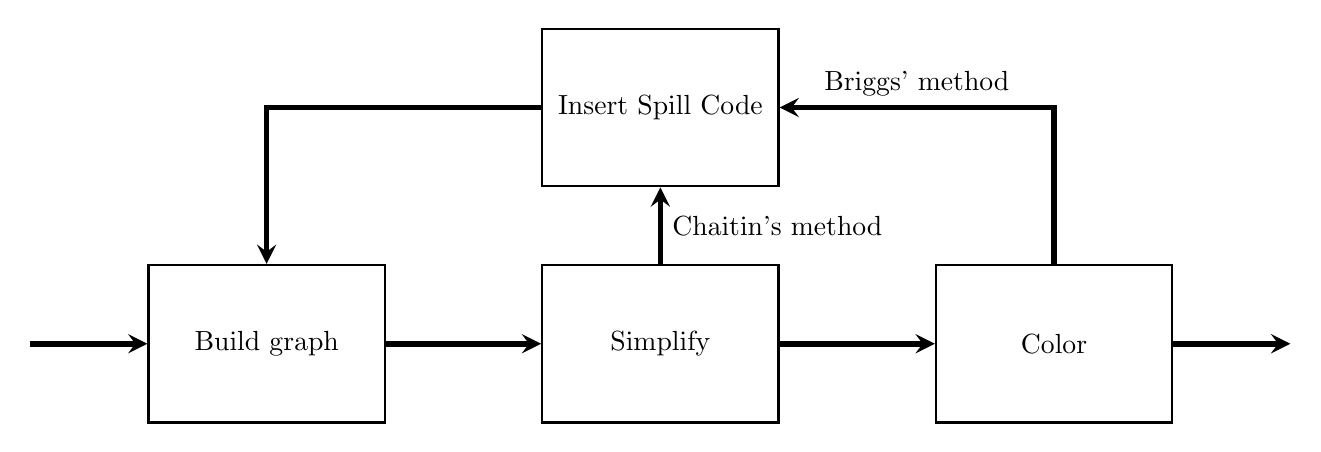
\begin{tikzpicture}[auto,
			    box/.style={inner sep=0mm,minimum height=2cm,minimum width=3cm,draw},thick,
			    edge/.style={->,>=stealth,line width=2pt},
			]
	    \node[box] (build) at (0,0) {Build graph};
	    \node[box] (simplify) at (5,0) {Simplify};
	    \node[box] (color) at (10,0) {Color};
	    \node[box] (spill) at (5,3) {Insert Spill Code};

	    %start
	    \draw [edge,->] (-3,0) -- (build.west);

	    %loop
	    \draw [edge,->] (build.east) -- (simplify.west);
	    \draw [edge,->] (simplify.east) -- (color.west);
	    \draw [edge,->] (simplify) -- node [swap] {Chaitin's method} (spill);
	    \draw [edge,->] (color) -- (10,3) -- node [swap] {Briggs' method} (spill.east);
	    \draw [edge,->] (spill.west) -- (0,3) -- (build);

	    %end
	    \draw [edge,->] (color) -- (13,0);
	\end{tikzpicture}
	\caption{Register allocation phases of Briggs and Chaitin \cite{briggs}.}
        \label{chaitin-briggs}
	\end{figure}

\subsection{Chow Hennesy}
Chow-Hennesy assume that all variables reside in memory and are loaded into registers as required. This is the reverse concept of Chaitin and Briggs. A \textbf{priority function} is used to calculate the saving when a variables is kept in a register instead of the memory. The \textbf{variables which have the greatest savings} are then selected to be stored in registers. Chow-Hennesy's register allocator works on \textbf{procedure level}. The priority based register allocation algorithm determines priorities for register-residing candidates using estimates derived from the program and from machine parameters. Because it does not backtrack, the running time is good regardless of colorability. If no suitable register is found (i.e. the algorithm cannot assign a color to the next highest priority), then live range splitting is applied and each smaller live-range can be assigned to a different register.\\

Parameters that are important for the priority algorithm
\begin{itemize}
	\item Execution time costs and savings due to register assignments (load, update, stores), which indicate how much faster the given code segment will execute when the variables are put into registers. (memory-to-register, register-to-memory moves
    \item time saved for referencing a variable in a register
    \item execution frequency of variable (live ranges extending loops have greater priority)
\end{itemize}


Steps in the Chow-Hennesy algorithm:
\begin{enumerate}
	\item Separate the \textbf{unconstrained live ranges} to handle them in the last step. Unconstrained live ranges are those which have less neighbors than available registers.
	\item Repeat steps a) to c), each time assigning a color to a live range until all constraint live ranges have been assigned a color or until there is no register left that can be assigned to any live range in any basic block.
 \begin{enumerate}
	\item Compute the priority function $P(lr)$ for each constraint live-range lr if has not been computed. If $P(lr)$ is negative, or if $lr$ is uncolorable, mark $lr$ as a noncandidate, and leave it unassigned. Delete $lr$ from the interference graph so that live ranges interfering with it will have on less interference.
	\item Find the live range with the highest priority function, $lr*$, and assign a color to it. The color must not be in the \textbf{forbidden} set for $lr*$. The forbidden set lists registers that are not allowed as target registers for the given live range. For each live range that $lr*$ interferes with, update the \textbf{forbidden} information.
	\item Check each live range interfering with $lr*$ to see if it needs to be split. A live range needs to be split if all of its target registers are in its forbidden set (forbidden set equals the set of available registers).
 \end{enumerate}
	\item Assign colors to the unconstrained live ranges, each time choosing a color not belonging to their forbidden set.
\end{enumerate}

\paragraph{Priority function:} The priority function $P(lr)$ is a measure of the relative benefits of assigning a given live range to a register and proportional to the total amount of execution-time savings $S(lr)$ gained due to the live ranges residing in register. It assigns a priority to each live range $lr$ to determine if it should be allocated to a register. $P(lr)$ is computed as the sum of execution time savings divided by the number of units in each live range:
\begin{align}
s_{i} &= LOADSAVE \times u + STRSAVE \times d - MOVCOST \times n\\
S(lr) &= \sum_{i\in lr}{s_i \times w_i}\\
P(lr) &= \frac{S(lr)}{N}
\end{align}
with
\begin{itemize}
	\item $s_i$ = Weighted sum of load costs, where $u$ is the number of uses, store costs, where $d$ is the number of definitions, and move costs, where $n$ is the numer of register moves needed in that live unit, per unit. A unit is normally a basic block.
	\item $w_i$ = Estimated execution frequency
	\item $N$ = Number of live units in the live range (=size of the live range). The bigger it is, the more register resources it takes. Smaller live ranges with the same amount of total saving have higher priority.
\end{itemize}

So the priority function is an estimate of the total register savings normalized by the size of the region occupied. A live range in which the occurrences are spread evenly should be favored over ones where the occurrences are concentrated into small regions. In a live range with uneven occurrences it is good to delay assigning it a register so as to leave open the possibility that only the heavily clustered portion be allocated to register, in case of a run out of registeres in the later part of the coloring process.

\paragraph{Live range splitting:} If a symbolic register has a very long live range it can be split into two parts, this way each smaller live range can be spilled separately if necessary. Live range splitting can be easily added to Chaitin and Briggs but was not present in the original algorithms. Live range splitting can cause the constrained and unconstrained pools (Chow) to change. Chow separates a component of the original live range that is as large as possible to the extent that its basic blocks are connected to avoid creating too small live range fragments.

\subsection{Differences and related concepts}
Besides knowing the algorithms, it is important to know some of their differences. The following differences between the algorithms have been emphasised in the lecture. Additional differences can be found in the paper of Chow-Hennesy, which contains a summary of the differences between Chaitin and Chow-Hennesy's algorithms (see \cite{chowhennesy}, Section 6).

\begin{itemize}
	\item Chaitin vs Chow: Most important differences arise from the timing of register allocation with respect to code generation \\

    	\begin{itemize}
        	\item Chaitin: allocates registers after the final form of the code is known; uses machine level instructions as units for coloring; Units are smaller (use of machine instruction level within each basic block) and therefore has more candidates; live ranges span only part of the basic block and the chromatic number is smaller; On machine instruction level all registers can participate in coloring; Maps unlimited number of symbolic registers to "real" machine registers; Never splits live ranges and lowers the chromatic number\\interferences by spilling - a live range is either colored or spilled; Cost function is used to find variable which is least costly to spill; colors are assigned in a reverse-order backwards pass; Spilled node is removed from interference graph and needs to be reloaded at each use and it has to spill multiple times until the graph can be colored; requires more memory and processing overhead
            \item Chow: allocates registers using an intermediate representation and before code generation; uses basic blocks as unit for coloring; Because of the bigger units there are less candidates to be colors; the interference graph is smaller and it's maybe no as effective but faster; On intermediate code-level special purpose registers must be excluded, all variables have home locations and variables are identified which should be promoted to registers; split live ranges to lower the number of interferences and either assign different colors or leave one of them unallocated; Cost/priority function is used according to their benefits of residing in registers; Coloring in one single forward pass; Does not spill and leaves variable in home location;
        \end{itemize}
	\item With Chow, all variables reside in memory initially and the register allocator chooses individual live ranges to allocate to registers. Therefore the code generator includes extra code to access them. Chaitin and Briggs hold all live ranges as symbolic registers and spill a live range to memory only when the symbolic registers cannot be mapped to a real register (i.e. the chromatic number is too high)
	\item Both Chaitin and Briggs algorithms need multiple iterations where as Chow-Hennesy finishes in one iteration. The reason is that for Chaitin and Briggs the insertion of spill code may block additional registers thus requiring more live ranges to be spilled (see Figure \ref{chaitin-briggs}).
	\item Chaiting and Briggs do the life range analysis on instruction level where as Chow-Hennesy perform life range analysis on basic block level. This is because Chaitin and Briggs do register allocation after instruction selection, but Chow-Hennesy's algorithm works on the intermediate code level.
	\item Chaitin and Briggs do register allocation for all registers, where as Chow-Hennesy only do register allocation outside of basic blocks.
\end{itemize}

The following paragraph summarizes some concepts that are relevant in connection with register allocation.

\paragraph{Calling conventions:} Calling conventions are conventions about how registeres are used and who is responsible to save and restore them. There are \textbf{caller-saves} and \textbf{callee-saves} registers. The conventions are a result of a multi-step proceedure. First the architecture has an impact on the calling conventions, then the operating system and lastly the used programming language. Calling conventions are part of the ABI and if not taken care of they my cause incomparibilities between programm binaries such as if libraries are used or programms written in different languages interact.\\
With caller-saved registers the caller is responsible for saving their contents before procedure calls and restoring their contents after return from calls.\\
With Callee-saved registers, the caller regards (betrachten) the registers contents as being undisturbed across a procedure call. A procedure that uses a callee-saved register mst save its contents at procedure entry and restore it before exit.\\
The parameter registers and function return registers must be caller-saved when they are used to keep variables between calls. The classed of registers have to be treated differently in the register allocation process if the allocation has to be optimal.


\paragraph{Pre-coloring:} Pre-coloring is used to assign correct colors to argument registers to avoid unnecessary copy instructions.

\paragraph{Rematerialization:} Some optimizations in Section\, \ref{sec:optimization}\, such as \textit{common subexpression elemination} optimize a program by removing redundant computation. The disadvantage of such an optimization can the that more symbolic registers are used or that the live range of a symbolic register is increased. However sometimes it can be cheaper to recompute a value than to store it in a register. This is often the case if a value can be recomputed with a single instruction. Rematerialization recomputes a value from another value such that instead of two values only one value needs to remain in a register and the other can be recomputed when needed. Rematerialization is often used in address calculation such as adding a constant value to an address. For example in \lstinline|*p = *q + 2;|, if $p$ is used at different locations in a function it can either remain in a register or be recomputed from $q$ each time it is needed. Rematerialization is commonly done by register allocators when it is easier to recompute a value, than to keep it in its own register or to reload it from memory.

\section{Coalescing}
Coalescing is the process of merging of live ranges (i.e. putting variables in the same register) which do not interfere in the interference graph by eliminating copy-instruction (i.e. coloring the source and the target of the copy instruction with the same color and \textbf{union their edges} in the interference graph). Mostly it is done if one life range ends and another begins and they are separated by a copy-instruction.
Coalescing may affect the colorability of an interference graph, both negative and positive results are possible.\\
Negative: It can yield a graph with nodes of higher degrees, because the coalesced node has the union of the edges from the source and the target.\\
Positive: If a node interferes with both the source and the target being coalesced, the degree of this node is reduced by one.\\
The target of coalescing is to minimize the spill cost while maximizing the number of coalesced copies.
\begin{itemize}
	\item \textbf{Aggressive coalescing} (used by Chaitin): It coalesces any pair of non-interfering copy-related nodes and therefore removes all possible copy instructions. This process achieves the best result of copy elimination by fully exploiting the positive impact but has probably the worst spill and totally ignores negative impacts. It does not ensure that colorability is preserved. But overall the positive impact of aggressive coalescing overweigh the negative ones.
	\item \textbf{Conservative coalescing} (Used by Briggs): Performs safe coalescing only when graph colorability is not affected. \textit{``For given two nodes $x$ and $y$, if the coalesced node $xy$ has less that K significant-degree neighbors, $xy$ does not change the colorability of the interference graph``''}. Was intended to be an improvement but later analysis showed that the algorithm actually performed worse than aggressive coalescing. Colorability is preserved (Significant neighbor means a node with degree greater than the number of registers). A conservative coalesced node is never spilled.
	\item \textbf{Iterative coalescing}: It performs conservative coalescing iteratively and eliminates more copies by interleaving conservative coalescing with a coloring simplification phase which increases the chances of conservative coloring. Also has worse results than aggressive coalescing. Is not really better than conservative coalescing. Colorability is preserved. (Gutes Beispiel in [14], Seite 169 linke Spalte)
	\item \textbf{Optimistic coalescing}: Does aggressive coalescing of all pairs of non-interfering nodes. But the algorithm memorizes what has been coalesced (to make live range splitting possible) and spilling must be controlled. When a coalesced node must be spilled, it is split back (\textit{live range splitting}) into separate nodes to reduce spill cost and giving up coalescing, i.e. if coloring is not possible and nodes need to be spilled, then the coalescing is reversed by live range splitting and then only parts of the nodes are spilled if possible. There is a better chance of coloring one (preferably the one with higher spill cost) of them without affecting the rest of the coloring and it leads to reduced spill costs. But it can also be the case that none of them or both of them can be colored separately. (Beispiel in [14] S. 170 linke Spalte). It has the \textbf{best results} and removes almost as much copy-instructions as the aggressive algorithm and generates the smallest number of spill instructions. \textit{split back means} that if two nodes $x$ and $y$ are coalesced, they are split up again - undo of coalescing. If live range splitting has to be done in a graph with coalescing, it is suggested to use a coalesced node and if there are more coalesced nodes, then the one with more nodes, i.e. prefer $xyz$ (coalescing of three nodes) over $uv$. (Bsp in [14] S 170 rechte Spalte)
\end{itemize}

Conservative coalescing has been introduced, because the aggressive can return bad results. But it turned out that it can be/or is even worse than aggressive coalescing. The improvement was a "verschlecht-besserung".\\
Conservative and iterative heuristics attempt to avoid negative impacts but they give up coalescing too early and lose many opportunities that would turn out to be safe. They ignore the fact that coalescing may improve the colorability of the graph, e.g. $x$ interferes with both the source and the target nodes being coalesced. The number of edges of $x$ would be reduced by one after coalescing. (Bsp in [14], Seite 169 rechte Spalte)

\section{Optimal register allocation using integer linear programming}
Performance overhead of spill code is minimized by using integer linear programming to achieve near optimal results. Since the problem is
NP-complete an optimal solution will be instractable for very complex problems. However the Optimal Register Allocator (ORA) solver still
produces very good results that are very often within 1\% of the optimal solution. However in order to define what optimal means we need
to know which optimizations are being done (or not done) by the register allocator.\\

\noindent \textbf{What does the register allocator do and not do?}
\begin{enumerate}
 \item The register allocator does not reorder instructions.
 \item The register allocator adds only spill load instrucitons, spill store instrucitons, and rematerialization instructions.
 \item The register allocator removes only copy instructions and instructions defining symbolic registers that are rematerialized.
 \item All controll-flow paths throguh a function can potentially execute.
 \item At a given location, the cost of a spill instruction is a fixed number of cycles (based on the instrucitons' type) times the
       location's estimated execution count.
 \item A basic block's estimated execution conut equals the sum of the countes exeiting the block, i.e. estimated execution counts
       satisfy Kirchhoff's current law over the control flow graph.
\end{enumerate}

The ORA implementation is composed out of three modules. The analysis module analyzes a functions control flow graph and identifies
points which require a decision about register allocation actions. For each decision a boolean decision variable is introduced that
records if the decision is made (1) or not (0) and also what action is taken if the variable is set to 1. These decision variables are
then build into a series of \textbf{inequalities} that model constraints for the decision variables. The solver module then solves these
inequalities and finally the rewrite module rewrites the code according to the results in the decision variables.

\subsection{ORA Modules}
Most of the paper focuses on the \textbf{analysis module} and explains the steps to derive (in)equalities from decision variables. The
steps in the analysis module are as follows:

\begin{itemize}
 \item Use live range analysis on the functions control flow graph and build an \textbf{instruction graph} for each symbolic register.
       The instruction graph contains solid and dashed lines for each symbolic register to show active and inactive live ranges,
       respectively.
 \item Apply transformations to create a \textbf{symbolic register graph}. Each transformation can potentially create one or more
       conditions. A \textbf{condition} is an equality or inequality function containing decision variables to constrain the valid
       assigments to the decision variables. The following gives an example for such a condition:
       \begin{align}
        x_{defA} &= x_{use-end1A} + x_{use-cont1A}
       \end{align}
       This condition ensures that if the symbolic register $A$ is allocated to a register at the given instruction, then its use must
       either end at that point or it must continue. At this point decision variables are not yet tied to real registers, that happens
       in the next step.
 \item A copy of each symbolic register graph and its associated set of conditions is made for each \textbf{real register} that is
       available for allocation. For example:
       \begin{align}
        x^1_{defA} + x^2_{defA} &= 1
       \end{align}
       This condition requires that the symbolic register $A$ is allocated to exactly one physical register, either register $1$ or
       register $2$, but not to both or none.
 \item Next several additional conditions are added to ensure that the solution is correct and optimal. For example conditions are
       added such that not too many or too few symbolic registers are allocated to real registers, or to ensure optimal spill code
       placement.
 \item Another additional transformation is for rematerialization. If a symbolic register can be rematerialized (see Section
       \ref{sec:register-allocation}), then the register allocator adds conditions to allow rematerialization instead of spilling
       and loading a symbolic register.
\end{itemize}

When all conditions have been created they are passed to the solver module to find a valid solution for all decision variables.

\subsection{Results}
The experimental results show that the ORA performs significantly better than other register allocators and is able to remove many
copy instructions and reduce the overhead of spill code significantly. There exists a second paper that was written six years later and
discusses improvements to the original ORA implementation. The authors were able to reduce the complexity of the algorithm
from $n^3$ to $n^{2.5}$. They also improved the speed by a factor of 1000x (10x CPU, 10x better solver, 10x improved model).


\section{Interproceedural register allocation}
Interproceedural register allocation (which is also often called global register allocation) performs register allocation accross procedures or compilation units and not just within a single function as is done in global register allocation. This solves the problem that different functions may assign the same global variable to different registers or the same register to different local variables, which causes unnecessary copy instructions.

\subsection{Global Register allocation at link time (Annotation based)}
The register allocation is delayed until link-time (to know what the other modules look like). A compiler produces object modules that can be linked and run without global register allocation. For each module there is a description, how it uses variables and procedures. The allocator then selects most frequently used variables and puts them into registers. Problems with ``normal'' (e.g. Chaitin, Briggs,...) allocation can occur one uses separate compilation, if one procedure calls the other, one must save and restore locals around the call, in case the other procedure uses the same registers for its own locals or if two procedures allocate the same global variable to different registers. It also creates a call-graph.\\

Allocation at link time keeps global variables in the same registers for all procedures and if one procedure calls another, it keeps the locals of both in different registers that they don't have to save and restore them around the call. The compiler does as much work as possible and generates code that can be linked and executed, but it includes extra information. With this extra information each module is rewritten.\\

Global here means interprocedural across all compilation units. The register allocation is split into three parts:
\begin{itemize}
 \item Compiler: Annotates Code so that it can be rewritten after register-allocation and collects usage information that a call graph can be built.
 \item Register allocator
 \item Linker/module rewriting
\end{itemize}

The  \textbf{compiler does as much work as possible} in order to maximize the benefits of seperate compilation such that in the linking phase there is not too much work required. The compiler inserts annotations into the object code which describe how variables are used (e.g. ``register actions`` that explain how the operands and results are related to the candidates for global register allocation). Annotations provide information to the linker about how to replace variables and how to rewrite the code. The following six annotations are inserted by the compiler. Each annotation is tied to a variable $v$. When the linker is run, it analyses the object code to identify if $v$ has been assigned to a register. If $v$ is in a register then the corresponding action (to an instruction) is applied, otherwise the annotation is ignored. (Bsp in [17] S. 208 linke Spalte)

\begin{itemize}
 \item \makebox[4.3cm]{REMOVE.v\hfill} Remove the instruction (e.g. corresponding instr: $r1 := load v$)
 \item \makebox[4.3cm]{STORE.v\hfill}  Replace store by copy instruction
 \item \makebox[4.3cm]{LOAD.v\hfill}   Replace load by copy instruction
 \item \makebox[4.3cm]{OP1.v, OP2.v, RESULT.v\hfill} Replace operands or result by register
\end{itemize}

The register allocator generates a call graph and uses the information provided by the compiler assign variables to registers. It does this by building groups of variables that are not active at the same time and then assigns a usage frequency to those groups. The same happens for global variables. Finally the groups with the highest freuqencies are allocated to registers. After variables have been assigned to registers the linker can use this information rewrite the code and to apply the actions that have been stored in the annotations. While doing this it must take care to adjust addresses of instructions or data if a previous instruction is being removed.

Additional considerations concern initialization and recursion.

\subsubsection*{Initialization}
Special care must be taken to initialize global variables and proceedure parameters. For global variables an INIT action is placed at the beginning of the program and runs when the program is invoked. The INIT action contains instructions to copy the initial value of global variables from memory to the respective register.

\subsubsection*{Recursion and indirect calls}
Recursion means that the same proceedure my be called repeatedly befor the first invokation has been completed. Therefore the program needs to take care to save the necessary registers of local variables before the next invokation of the proceedure. The question is who should be responsible to save the local varibles of the proceedure. It turns out that it is not enough if each recursive proceedure is responsible to save its local variables because this would not archive local variables of other proceedures in the call chain. The solution is to let the proceedure that makes the recursive call save the local variables of all proceedures in the call chain. The same
solution is used for indirect calls.

\subsection{Register allocation across procedure and module bounaries (Web)}
This has two important parts, the web algorithm itself and clustering (e.g. spill code motion).
\subsubsection*{Web algorithm:}
Performs several steps:
\begin{enumerate}
 \item Reads in source files and produces intermediate representation files.
 \item Creates program database.
 \item Uses Program database and transforms intermediate representation files into object files.
 \item Linking of the object files.
\end{enumerate}
The web algorithms creates a table with L\_REF, P\_REF, and C\_REF entries from which a web interference graph is generated. This is then
used to apply a coloring on the graph that determines which register is being used for each global variable.

\subsubsection*{Clustering (Splill code motion):}
The idea is to move spill code for callee-saved registers inside a cluster from one node to
its dominating node. If the node is being called more than once, then the overhead of the spill code is reduced. Same for caller-saved
registers which are moved down to lower nodes in the same cluster.

\section{Instruction Scheduling}
Instruction scheduling is an optimization that deals with rearranging the instructions of a program to better exploit the inherent
parallelism of the instructions. The goal is to move instructions that depend on each other further appart and instead insert independent
instructions inbetween. This prevents that dependent instructions block the processor pipeline and allows a more instructions to execute
simultaneously. The simplest form of instruction scheduling is called list scheduling because from a list of possible instruction that
can be scheduled one with the highest priority is selected based on some kind of heuristic. There exist two papers that deal with list
scheduling which both present different heuristics for the problem. The list scheduling algorithms presented in the papers have a worst
case complexity of $O(n^2)$ needed to build the dependency graph. However in practice there exists also a linear time algorithm.

The improved \textbf{linear time algorithm} works as follows. The algorithms goes through each instruction and each time a register is
defined the algorithm saves which instruction defined the register. Each time a register is accessed the corresponding instruction can be
looked up and the algorithm adds a dependency to the graph. The only problem with this algorithm is that the initialization of the
corresponding data structure may be expensive. However this can be optimized when using virtual registers by storing from which
instruction to which instruction a basic block extends. Based on these limits it can be easily determined if an instruction is still
independent. Otherwise the datastructures would need to be rebuild for each basic block.

\subsection{Phase ordering problem:}
A problem between instruction scheduling and register allocation is that both optimizations can have negative effects on the other one,
thus it is difficult to decide what should be done first -- register allocation or instruction selection. This problem is called the
\textit{phase ordering problem}. The list scheduling algorithms below attempt different solutions but still perform both optimizations
separately. A better solution is discussed in the next Section which presents algorithms that perform instruction scheduling and register
allocation together at the same time.

The impact of each optimization to the other is as follows:
\begin{itemize}
 \item Register allocation serializes the code and removes opportunities for scheduling (less instruction level parallelism).
 \item Instruction scheduling increases the length of the live ranges (register pressure), causing more interferences and thus requires
       the use of more registers or increased spilling.
\end{itemize}

\subsection{Instruction scheduling for the IBM RISC System/6000 Processor (IBM)}
The algorithm which is described in this paper performs the instruction scheduling twice, once before register allocation and once
afterwards. The first instruction scheduling has more freedom since register allocation has not yet been done, but register allocation
may insert spill code and delete move instruction which make a second run of instruction scheduling necessary. The algorithm itself works
as follows:
\begin{itemize}
 \item It uses a dependency graph which is constructed for each basic block. The dependency graph has one node for each instruction and
       adds a directed edge between two instructions if one needs to preceed the other.
 \item Edges are labeled with the delay between instructions.
 \item After the dependency graph has been build, nodes are labled upwards with the \textbf{maximum delay} from the node to the end of
       the basic block (red digits in Figure \ref{dependency-graph}).
 \item The algorithm keeps a \textbf{current time} counter, which is initially zero. It is increased by the execution time of each
       scheduled instruction, which is usually one.
 \item Nodes are labels with \textbf{earliest time} value which is calculated from the current time of the last scheduled predecessor
       plus the delay of that instruction to its successor. For example the node L.B has a delay of one and is scheduled in step 2 where
       the current time is increased to 2, so the ADD node would be labled with an earlies time of 3 (2+1).
\end{itemize}

Figure \ref{dependency-graph} shows the the dependency graph from the paper but adds the values of the maximum delay and a table that
shows how the current time is updated and which instruction is selected in each step.

\begin{figure}[h!]
\begin{tikzpicture}[node/.style={circle, draw, thick, minimum size=1.0cm,inner sep=0pt,font=\footnotesize,align=center},
		    item/.style={inner sep=0pt,font=\footnotesize,align=left},
		    edge/.style={->,>=stealth,line width=2pt},auto,
		    red/.style={draw=red},black/.style={draw=black},
		    legend/.style={draw=black}
		   ]
    \node[node]  (la) at 	(1, 7) {L.B 	\\ \textcolor{red}{1}};
    \node[node]  (lc) at 	(3, 7) {L.C 	\\ \textcolor{red}{1}};
    \node[node]  (ld) at 	(4, 5) {L.D 	\\ \textcolor{red}{1}};
    \node[node]  (le) at 	(8, 3) {L.E 	\\ \textcolor{red}{4}};
    \node[node]  (add) at 	(2, 5) {ADD 	\\ \textcolor{red}{0}};
    \node[node]  (sub) at 	(3, 3) {SUB 	\\ \textcolor{red}{0}};
    \node[node]  (store) at 	(4, 1) {ST.A 	\\ \textcolor{red}{0}};
    \node[node]  (compare) at 	(8, 1) {CMP	\\ \textcolor{red}{3}};
    \node[node]  (branch) at 	(6, 0) {BC	\\ \textcolor{red}{0}};

    \draw[edge]  (la)      -- node [swap] {1} (add);
    \draw[edge]  (lc)      -- node        {1} (add);

    \draw[edge]  (ld)      -- node        {1} (sub);
    \draw[edge]  (add)     -- node [swap] {0} (sub);

    \draw[edge]  (sub)     -- node        {0} (store);
    \draw[edge]  (store)   -- node        {0} (branch);

    \draw[edge]  (le)      -- node {1} (compare);
    \draw[edge]  (compare) -- node {3} (branch);

    \node[legend] (foo) at (11,6) {
	\begin{tikzpicture}
	    \node[item] (step1) at (0,  0) {1. Current time: $0\rightarrow1$;\quad select L.E\\
					    2. Current time: $1\rightarrow2$;\quad select L.B\\
					    3. Current time: $2\rightarrow3$;\quad select CMP\\
					    4. Current time: $3\rightarrow4$;\quad select L.C\\
					    5. Current time: $4\rightarrow5$;\quad select L.D\\
					    6. Current time: $5\rightarrow6$;\quad select ADD\\
					    7. Current time: $6\rightarrow7$;\quad select SUB\\
					    8. Current time: $7\rightarrow8$;\quad select ST.A\\
					    9. Current time: $8\rightarrow9$;\quad select BC};
	\end{tikzpicture}
    };

    \node[legend] (foo) {
	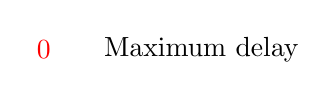
\begin{tikzpicture}
	    \node (redsquare) at (-2, -1) {\textcolor{red}{0}};
	    \node (redlegend) at (0, -1) {Maximum delay};
	\end{tikzpicture}
    };
\end{tikzpicture}
\caption{Dependency graph constructed by IBM instruction scheduling algorithm}
\label{dependency-graph}
\end{figure}

When deciding which node to select in each step, the algorithm uses an eight step heuristic. Since there is no planning or lookahead
involved the algorithm is not guaranteed find the best solution. There are the following seven heuristics:
\begin{enumerate}
    \item Initialize the set of all those instructions that have not yet been selected, and that have no predecessors in the dependency
          graph (these are the ''legal`` ones).
    \item Refine the subset to those instructions whose earliest time has arrived or, if none, those with the smallest earliest time.
    \item If one or more instructions have been selected, and if the current subset contains one or more instructions of opposite type
	  (fixed/floating) from the last one selected, then refine the current subset to those of this opposite type.
    \item Refine the subset to those of maximum total delay along the path of each instruction to the end of the basic block.
    \item Refine the subset to those of minimum ''liveness weight``.
    \item Refine the subset to those with greatest uncovering''.
    \item Refine the subset to the unique instruction that came first in the original ordering.
\end{enumerate}

\subsection{Efficient Instruction Scheduling for a Pipelined Architecture (HP)}
The general idea is similar to the IBM algorithm. The algorithm works as follows:
\begin{enumerate}
 \item Build a scheduling dag over the basic block
 \item Put the roots of the dag into a candidate set
 \item Select the first instruction to be scheduled based on the heuristics below
 \item While the candidate set is not empty do the following:
    \begin{enumerate}
    \item based on the last instruction scheduled and the heuristics select and emit the next instruction that should be scheduled
    \item delete the instruction from the dag and add any newly exposed candiates
    \end{enumerate}
\end{enumerate}

The following heuristics use the following criteria to determine the priority with which a candidate should be scheduled:
\begin{enumerate}
 \item Whether an instruction interlocks with any of its immediate successors in the dag.
 \item The Number of the immediate successors of the instruction
 \item The length of the longest path from the instructions to the leaves of the dag.
\end{enumerate}

The instruction scheduling in is performed before register allocation. The paper mentions register allocation but claims that
''serializing definitions does not unduly restrict [the] code``.

\section{Register allocation \& instruction scheduling}
This section introduces three methods which combine instruction scheduling and register allocation in order to solve the phase
ordering problem. The first paper presents two algorithms the Integrated Prepass Scheduling (IPS) and the dag-driven register allocation.
The second paper introduces a method named Register Allocation with Scheduling Estimate (RASE).

\subsection{Integrated Prepass Scheduling}
The main issue of the phase ordering problem is that register allocation reduces opportunities for scheduling while instruction scheduling
increases the length of live range making register allocation more difficult. The IPS algorith solves this problem by using two strategies
that can be selected depending on what strategy is more appropriate. The two strategies are:
\begin{itemize}
 \item CSP (Code scheduling for pipelined processors) reduces pipeline delays but can increase the lifetime of registers. It is used if
       enough free registers are available.
 \item CSR (Code scheduling to minimizes register usage) is used when the number of registers is low to control register usage. It tries
to ''find the next instruction which will not increase the number of live register or if possible, decrease that number``.
\end{itemize}
IPS uses a simple heuristic to switch between the two strategies, it keeps track of the number of available registers in a variable named
AVLREG, if the number of free registers drops below a certain threshold, then it switches to CSR. When AVLREG has increased above the
threshold then it switches back to CSP.

\subsection{Dag-driven register allocation}
Dag-driven register allocation is a form of postpass scheduling to keep the graph flat and wide. It also does not insert any
additional spilling instructions into the code. The algorithm introduces two measures for the graph the width and the height:
\begin{itemize}
 \item The \textbf{width} is defines as the maximum number of mutually independent nodes. Wider graphs indicate higher parallelism.
 \item The \textbf{height} is the length of the longest path. If the graph is too high then code scheduling becomes less efficient.
\end{itemize}
The goal of the dag-driven register allocator is to balance the dag. To do that it will \textbf{minimize the height} of the graph and
\textbf{limit the width} of the graph to a number that is less or equal to to the amount of registers available.

The dag-driven register allocator uses two techniques to achieve these goals:
 \begin{itemize}
  \item First, it makes use of free WAR dependencies. That is, it makes use of redundant dependencies when allocating registers. Such
        redundant dependencies can occur for example if a RAW dependency already exists between two instructions. In the Listing below
        assume registers \lstinline|R2| and \lstinline|R4| are available for reuse in the second instruction. There is already a RAW
        dependency for \lstinline|R5|, so when register \lstinline|R4| is choosen a redundant WAR dependency is added. This WAR
        dependency is free because of the existing RAW dependency for \lstinline|R5|, so \lstinline|R4| is a better choice than
        \lstinline|R2|. When reusing registers, the dag driven register allocator will prefer those registers that only introduce redundant dependencies.


\begin{lstlisting}[xleftmargin=3.5mm]
Add R5, R4, R1
Sub ??, R5, #4
\end{lstlisting}

  \item Second, it tries to balance the growth of the dag. When a register is reused and the register allocator cannot make use of a
        free WAR dependency then it must add a dependency which connects two independent paths and the height of the dag will be
        increased. So the important part in balancing the dag is to find a path to connect the path of the current instruction, such that
        it does not increase height of the dag too much. To achieve this for each instruction the \textit{earliest issue time (EIT)} and
        \textit{earliest finish time (EFT)} are computed. The register allocator now tries to find two paths such that one has a high
        EIT and the other has a large EFT.
 \end{itemize}

\subsection{Register Allocation with Scheduling Estimate (RASE)}
The RASE approach is an integrated scheduling and register allocation method. The idea behind RASE is to perform a pre-scheduling in
order to calculate schedule cost estimates that enable the register allocator to make a decision about how many registers it is going to
use. Essentially RASE splits the available registers into two parts, one part for the register allocator, and one part for the
instruction scheduler. The RASE algorithm has three phases:

\begin{enumerate}
 \item Pre-scheduling
 \item Global register allocation
 \item Instruction scheduling with local register allocation
\end{enumerate}

The \textbf{first phase} is the pre-scheduling, which calculates the schedule cost estimate. During the pre-scheduling, the order of the
instructions is not changed.

The \textbf{second phase} performs a \textit{global} register allocation using the schedule cost estimate, but leaves enough free
registers for the last phase. The schedule cost estimate allows the register allocator to estimate, how the cost of local register
allocation increases, if it uses more registers to allocate \textit{global} symbolic registers. In the second phase the register
allocator is only responsible for allocating global symbolic registers to physical registers, the allocation of \textit{local} symbolic
registers is defered until the third phase.

The \textbf{third phase} performs the instruction scheduling and does the \textit{local} register allocation.  This register allocation
must be within the limits for \textit{local} registers that have been determined in the second phase.

\textbf{How does the schedule cost estimate function work?} The schedule cost estimate is a quadratic function (of \textit{regressive}
form). It takes as input the number of local registers and returns as output the estimated machine cycles:
\begin{figure}[h!]
\begin{center}
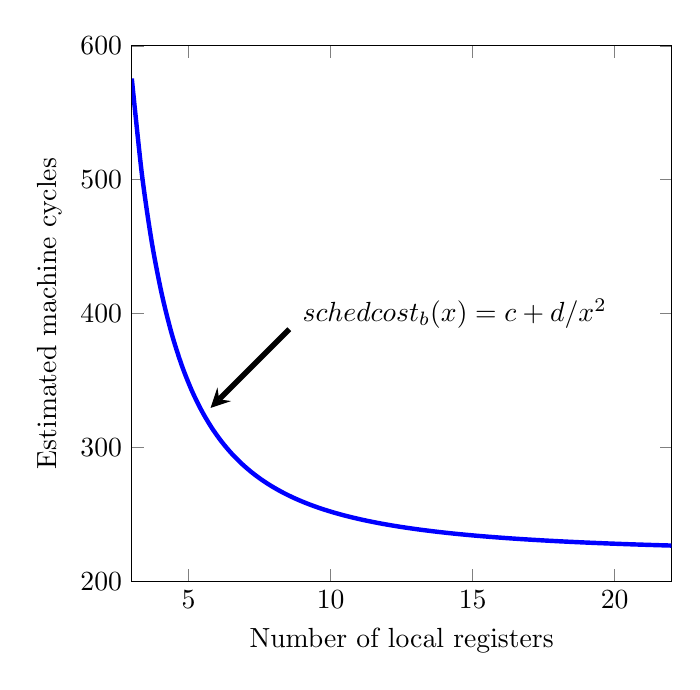
\begin{tikzpicture}
   %\draw[->] (-0.5,0) -- (4.2,0) node[right] {$x$};
   %\draw[->] (0,-0.5) -- (0,4.2) node[above] {$y$};

    \begin{axis}[xmin=3,xmax=22,ymin=200,ymax=600,samples=55,y=0.017cm,
                 xlabel={Number of local registers},
                 ylabel={Estimated machine cycles}]
     \addplot[blue, smooth, ultra thick, domain=3:22] (x,{220+3200/(x*x)});
    \end{axis}

   %\draw[scale=0.5,domain=1:8,smooth,variable=\x,blue] plot ({\x},{1 + (7 / \x^2)});
   \draw[<-,>=stealth,line width=2pt] (1,2.2) -- (2,3.2) {};
   \node (formula) at (4.1,3.4) {$schedcost_b(x)=c+d/{x^2}$};
\end{tikzpicture}
\end{center}
\caption{Schedule cost estimate function}
\label{schedule-cost-estimate-function}
\end{figure}

The coefficientes $c$ and $d$ are computed as part of the pre-scheduling. Essentially this function allows the register allocator to
estimate how much the required machine cycles are incresed, due to loss of parallelism, if the available local registers are reduced.
As can be seen in Figure \ref{schedule-cost-estimate-function}, if the register allocator leaves 15 registers to the third phase,
then the total execution cost for that basic block it not very high, however if only 4 or 5 registers are left to the third phase,
then the cost increases quite significantly.

\subsection{Which algorithm should be prefered?}
When comparing the three algorithms one can say that IPS is the ''best``
algorithm, because it is realively easy to implement and produces results which are comparable to the other two solutions. The IPS
algorithms can be easily implemented in existing register allocators such as Chaitin or Briggs. In contrast the DAG driven algorithm and
RASE are both quite complicated to implement but do not produce significantly better results.

\section{Trace scheduling}
Trace scheduling attempts to provide another solution for the phase ordering problem. A trace is \textbf{a sequence of instructions that
can have exit and entry points but that must not have any loops}. The trace
scheduler orders traces by their frequency and schedules the most frequent trace first. Inner most loops usually contain
the traces with the highest frequency and are thus scheduled first. Since the instruction scheduler is also responsible for assigning
variables to registers, this scheduling approach effectively gives priority to those variables, which are used with the highest frequency.
The advantage of this approach is that at the beginning all registers are available for use by the scheduler, giving the scheduler
complete choice over registers with the highest frequency.

Since traces are scheduled individually of each other care must be taken if two traces merge with each other or split from each other.
This can either happen at split nodes, when one trace leaves from the other, or at join nodes, when one trace joins into another. Since
the traces are scheduled and register allocated individually there needs to be a machanism to communicate register allocation decisions
between traces. This is done by adding special nodes named \textit{Value Location Mapping} (VLM).

\subsection{Variable Location Mapping (VLM):}
A VLM is placed at the split or join nodes between two traces and contains the information about already allocated variables. So when a
trace is scheduled that contains a variable which has already been allocated, then the scheduler can take this decision into account. It
tries to ensure that individually scheduled traces reference their values at the same locations to avoid unnecessary data motions such as
register moves, spills and restores. If a VLM appears at the beginning of a trace, then the scheduler must make sure to read values that
appear in the trace from the locations specified in the VLM. On the other hand, if a VLM appears at the end of a trace, then the
scheduler must make sure to \textit{satisfy} the references in the VLM, that is, it must store values that appear in the trace at the
locations specified by the VLM. Sometimes it may not be possible to satisfy the constraints in a VLM. This can happen if there is a VLM
both at the top and bottom of a trace and both VLMs have conflicting locations for the same variable. If it is not possible to satisfy
the location constraints in a VLM, then the scheduler must insert \textbf{compensation code} to move or copy values to the correct
locations.

\subsection{Delayed binding}
Delayed binding is used because some values have live ranges that go through a trace but the value is not actually used inside the
trace. \textit{''A delayed binding is a sort of pseudo-location that may be assigned to an unreferenced value by the instruction
scheduler.''} Delaying the variable binding until there is an actual reference to it helps to preserve registers for more important
values. When a delayed binding is bound to an actual location it is determined if there exists an unused register that is free through out
the whole live range of the value, otherwise the value is bound to memory.

\textbf{Paper Evaluation:} The evaluation of the trace scheduling paper is not useful, because the results are only compared to
themselves.

\section{Software pipelining}
Software pipelining is a form of instruction scheduling with the goal of scheduling the different instructions of a loop in a way, such
that multiple loop iterations can be active at the same time.

\subsection{Modulo Variable Expansion}
One problem in software pipelining is that a variable is defined and then used two cycles later. If
this variable remains in the same register during every loop iteration, then each iteration must take two cycles. However if copies of
the variable are kept in different registers for consequtive iterations, then it is possible to start a new operation in each cycle.
This concept of using multiple registers for the same variable is called \textbf{modulo variable expansion}.

%TODO: Which problems occur du? What is it? Why is it needed?

\subsection{Resource-constrained software pipelining}
This algorithm provides a solution to the software pipelining problem by combining instructions into sets of available instruction which
are then scheduled. The algorithm is very elegant but has the grave problem that the algorithm is only shown graphically, the actual
\textbf{heuristic} to choose which instructions can be combinede into the sets and how to schedule them \textbf{is missing} and thus the
algorithm cannot be implemented.

\subsection{Iterative modulo scheduling:}
Different scheduling strategies exist in software pipelining, the iterative modulo scheduling is a form of the ``schedule-then-move''
stategy. The goal of iterative modulo scheduling is to find a schedule for the instructions of a loop body, such that the loop
can be repeated at regular intervals, without causing any conflicts between the instructions. There are two types of conflicts that can
occur, a resource conflict or a dependency conflict:
\begin{itemize}
 \item Resource conflict: The same processor resource such a bus or a pipeline stage are in use at the same time.
 \item Dependency conflict: Can be an inter-iteration-dependency if there exists a dependency between instructions in two different
       iterations of a loop or an intra-iteration-dependency if there is a dependency between two instruction in the same loop iteration.
\end{itemize}
Before the actual iterativev modulo scheduling is performed several other optimizations and transformations are performed, one of them is
IF-conversion. \textbf{IF-conversion} removes all branches except the loop closing branch and converts the code into a single basic block. The different branches of the original code are instead expressed by data dependencies involving predicates.

Iterative modulo scheduling introduces the notion of an \textbf{initiation intervals (II)} which is the interval between the start of a
new loop iteration. An II of four means that every 4-th instruction a now loop iteration begins. A \textbf{minimum initiation interval
(MII)} is calculated and used to calculate the minimum length of a schedule. To compute the actual II a
candidate II is used that is initialy set to the MII and then step wise incremented until a suitable II is found. The MII is the maximum
of the Resource constraint MII and Recurrence constraint MII values:

\begin{itemize}
 \item The \textbf{Resource-constrained MII} used to avoid that two instructions block the same processor resource at the same time. For
       example if an add instruction requires to use the result bus in the fourth cycle and a multiply instruction requires the result bus
       in the sixth cycle, then an add cannot be sheduled two cycles after a multiply. The ResMII can be computed by performing a
       bin-packing of the reservation tables for all the operations.
 \item The \textbf{Recurrence-constrained MII} is used prevent data dependencies between the same operations in different loop iterations.
       % TODO: How does this work?
\end{itemize}

The iterativ modulo scheduling starts with the initially computed II and tries to find a valid schedule for this II and a given budget. If
no schedule can be found the II is increased by one and the proceedure is repeated until a schedule is found. There are some differences
between the traditional acyclic list scheduling and iterative modulo scheduling:
\begin{itemize}
 \item Instructions can also be unscheduled and rescheduled, thus operation scheduling instead of instruction scheduling is performed.
       Operation scheduling picks an instruction and scheduls it at a time slot that is both legal and most desirable.
 \item Instructions do not become ``ready'' after their predecessors have been scheduled. Instead the algorithm keeps track of which
       instructions have never been scheduled and schedules instruction based on a priority function.
 \item If an instruction is unscheduled it is immediately rescheduled.
\end{itemize}

\subsection{Optimizations for processors with SIMD instructions}
Processors with SIMD instructions allow to execute the same sequence of instructions on multiple instances of data such as arrays. For
this purpose the data must be naturally aligned on the block size. If the alignment cannot be statically determined at compile time
then the compiler needs to insert dynamic runtime checks that verify if the pointers are aligned. If the pointers are aligned then
SIMD instructions can be used, otherwise the memory is accessed sequentially. These dynamic checks increase the program size and impact
the execution speed. Not only the dynamic checks increase program size, but also the fact that there need to be two versions of a loop,
one version with SIMD instruction and another version which accesses memory locations sequentially.

The paper describes an algorithm to generate SIMD instructions for logical and arithmetical operations as well as SIMD load and
store instructions. Further more it describes an analyzation technique to statically identify the alignment of C pointers.
This alignment information can then be used to reduce dynamic alignment checks and thus reduce the overhead of those checks.
About 50\% of all pointers can be statically identified.

\subsubsection{SIMD Instruction Generation}
The SIMD instruction generation consists of two phases:
\begin{itemize}
 \item Phase 1 deals with the generation of logical and arithmetical SIMD instruction inside loops that process arrays.
 \item Phase 2 deals with the generation of LOAD and STORE SIMD instructions for data that is used by the logical and arithmetical SIMD
       instructions which have been generated in phase 1.
\end{itemize}

In order to generate logical and arithmetical SIMD instructions from loops the \textbf{loop must be unrolled $k$ times}, where $k$
depends on the number of elements in a SIMD instruction. For example if a loop processes 16bit elements and the SIMD operands are 32bit
then the loop needs to be unrolled two times. If the loop count is not a multiple of $k$ then a pre- or postloop is added which is
executed $N \mod k$ times, where $k$ is the unroll count and $N$ the loop count. Depending on the alignment information a preloop or
a postloop is added.

The main reason for loop unrolling is get an \textbf{acyclic dependency graph} for the loop body which contains enough equivalent
expressions that can be combined into a SIMD instruction. The nodes in the graph are \textit{s-nodes} (statement nodes) and
\textit{b-nodes} (groups of basic blocks). The algorithm first schedules s-nodes that are not candidates\footnote{Candidates are
those nodes for which SIMD instructions are available on the platform. For example if the target processor does not support a special
SIMD instruction for multiplication then nodes with multiplications are not candidates for SIMD instructions.} for SIMD instructions
as well as all b-nodes. Then it tries to find a series of s-nodes which are structurally equivalent and combines them into a SIMD
instruction. To identify the instructions that can be combined into SIMD nodes, the algorithm builds \textit{``all possible
combinations of SIMD candidates and rates them according to the number of resulting SIMD expressions and the number
of adjacent subwords in the SIMD expressions''}. Scheduled nodes are removed from the dependency graph and the proceedure is repeated
until the graph is empty.

The algorithm also applies scalar expansion and accumulator splitting. Scalar expansion replaces a scalar by an array which
contains copies of the scalar, such that it can be used with SIMD instructions. Accumulator splitting is used in reductions such as
calculating the sum of an array. The array is split into several smaller arrays for which the sum can be calculated in parallel, the
results is then a smaller array from which the final result can be computed.

\subsubsection{Alignment analysis}
The alignment analysis is done by \text{abstract interpretation} of the code. For each expression that modifies a pointer the
algorithm stores the possible remainders modulo $k$, where $k$ is the number of bytes in a SIMD instruction (e.g. 4 on 32bit). Doing
so keeps the possible state space small and prevents a state explosion during the abstract interpretation of the code.

The algorithm first performs an intra-proceedural analysis by examining pointers inside proceedures, followed by an inter-proceedural
analysis. When an array is defined or dynamically loaded, then the first element is already aligned correctly, that is the alignment
is zero modulo the block size. This is enforced by the program loader, the compiler and the function family of \lstinline|malloc|
when memory is allocated dynamically. When a pointer is modified for example through pointer arithmetic, the algorithm computes the
possible remainers of the new pointer. For example for a block size of 4 bytes the possible values for the pointer alignment are
\lstinline|{0,1,2,3}|. If the set of alignment information for a pointer contains only the value \lstinline|{0}|, then the pointer
is correctly aligned, if the set contains multiple values it means that that several alignments are possible. This in the next step
this aligment information is propagated accoss proceedure calls by the inter-proceedural analysis.

Based on the alignment information that the algorithm computed, dynamic checks are inserted if necessary.

\newpage
\begin{thebibliography}{9}
\footnotesize
\bibitem{powerpc}
The PowerPC 604 RISC Microprocessor (S.P. Song \& M.D. Denman), 1994

\bibitem{alpha}
Alpha AXP Architecture (R.L. Sites), 1993

\bibitem{intelp6}
Discorvery 6 - Intels Sternenschiff P6 im Detail (G. Schnurer), ct' 4/1995

\bibitem{compileroptimization}
Advanced Compiler Optimizations For Supercomputers (D.A. Padua \& M.J. Wolfe), 1986

\bibitem{convexfortran}
The CONVEX FORTRAN 5.0 Compiler (R. Mercer), 1988

\bibitem{globaloptimizer}
Effectiveness of a Machine-Level, Global Optimizer (M. S. Johnson \& T.C. Miller), 1986

\bibitem{iburg}
Engineering a Simple - Efficient Code Generator Generator (C.W. Fraser, D.R. Hanson, T.A. Proebsting), 1992

\bibitem{beg}
BEG - a Generator for Efficient Back Ends (H. Emmelmann, F-W. Schr\"oer, R. Landwehr), 1989

\bibitem{pbqp-instruction-selection}
Generalized instruction selection using SSA graphs (Andreas Krall et all.), 2006

\bibitem{briggs}
Coloring Heuristics for Register Allocation (P. Briggs, K.D. Cooper, K. Kennedy, L. Torczon), 1989

\bibitem{chaitin}
Register Allocation \& Spilling via Graph Coloring (G.J.Chaitin), 1982

\bibitem{chaitin2}
Register Allocation via Coloring (G.J.Chaitin, M.A. Auslander, A.K. chandra, J. Cocke), 1980

\bibitem{chowhennesy}
The Priority-Based Coloring Approach to Register Allocation (F.C. Chow \& J.L. Hennessy), 1990

\bibitem{coallescing}
Optimistic Register Coalescing (J. Park \& S-M. Moon), 1998

\bibitem{optimalregisterallocation}
Optimal and Near-optimal Global Register Allocation Using 0-1 Integer Programming (D.W. Goodwin \& K.D. Wilken), 1996

\bibitem{fasterora}
A Faster Optimal Register Allocator (C. Fu \& K. Wilken), 2002

\bibitem{annotations}
Global Register Allocation at Link Time (D.W. Wall), 1986

\bibitem{web}
Register Allocation Across Proceedure and Module Boundaries (V. Santhanam \& D. Odnert), 1990

\bibitem{instructionschedulingibm}
Instruction scheduling for the IBM RISC System/6000 processor (H.S.Warren), 1990

\bibitem{instructionschedulinghp}
Efficient Instruction Scheduling for a Pipelined Architecture (P.B. Gibbons, S.S. Muchnick), 1986

\bibitem{ips}
Code Scheduling and Register Allocation in Large Basic Blocks (J.R. Goodman \& W-C. Hsu), 1988

\bibitem{rase}
Integrating Register Allocation and Instruction Scheduling for RISCs (D.G. Bradlee, S.J.Eggers, R.R. Henry), 1991

\bibitem{tracescheduling}
Phase Ordering of Register Allocation and Instruction Scheduling (S.M. Freudenberger \& J.C. Ruttenberg), 1991

\bibitem{modulovariableexpansion}
Software Pipelining: An Effective Scheduling Technique for VLIW Machines (M. Lam), 1988

\bibitem{realisticsoftwarepipelining}
A Realistic Resource-Constrained Software Pipelining Algorithm (A. Aiken, A. Nicolau), 1990

\bibitem{moduloscheduling}
Iterative Modulo Scheduling: An Algorithm For Software Pipelining Loops (B.R Rau), 1994

\bibitem{simd}
Compiler optimizations for processors with SIMD instructions (I. Pryanishnikov, A. Krall, N. Horspool), 2006

\end{thebibliography}

\end{document}
